\documentclass[conference]{IEEEtran}
\IEEEoverridecommandlockouts
\usepackage[utf8]{inputenc}
\usepackage[T1]{fontenc}
\usepackage[spanish,es-tabla]{babel}
\usepackage{cite}
\usepackage{amsmath,amssymb,amsfonts}
\usepackage{algorithmic}
\usepackage{graphicx}
\usepackage{textcomp}
\usepackage{xcolor}
\usepackage{booktabs}
\usepackage{multirow}
\usepackage{array}
\def\BibTeX{{\rm B\kern-.05em{\sc i\kern-.025em b}\kern-.08em
    T\kern-.1667em\lower.7ex\hbox{E}\kern-.125emX}}

\begin{document}

\title{Análisis Comparativo de Técnicas de Optimización Convexa y No Convexa para Diagnóstico de Cáncer de Mama: Estudio Experimental con Dataset de Wisconsin}

\author{\IEEEauthorblockN{Mario Wilfredo Ramirez Puma}
\IEEEauthorblockA{\textit{Universidad Nacional del Altiplano - Puno} \\
\textit{Escuela Profesional de Ingeniería Estadística e Informática}\\
Puno, Perú \\
maramirezp@est.unap.edu.pe}
}

\maketitle

\begin{abstract}
Este estudio presenta una comparación experimental entre técnicas de optimización convexa y no convexa aplicadas al diagnóstico de cáncer de mama utilizando el dataset de Wisconsin \cite{wolberg1995}. Se implementaron seis algoritmos: tres convexos (Regresión Logística, SVM Lineal, Regresión Ridge) y tres no convexos (Redes Neuronales, SVM RBF, Algoritmos Genéticos). Los resultados revelan un empate técnico entre SVM Lineal y SVM RBF alcanzando 98.25\% precisión, con diferencias en eficiencia computacional favoreciendo métodos convexos \cite{boyd2004}. El hallazgo principal demuestra que el dataset es linealmente separable. Los métodos no convexos fallaron en superar a sus contrapartes lineales, validando el principio de parsimonia algorítmica.
\end{abstract}

\begin{IEEEkeywords}
optimización convexa, diagnóstico médico, aprendizaje automático, cáncer de mama, SVM, algoritmos genéticos
\end{IEEEkeywords}

\section{Introducción}

El diagnóstico temprano del cáncer de mama constituye un desafío crítico donde la precisión algorítmica impacta directamente la supervivencia del paciente. La selección de técnicas de optimización para sistemas de diagnóstico asistido representa una decisión fundamental que equilibra precisión, eficiencia e interpretabilidad clínica.

Este estudio aborda una pregunta central: ¿cuándo se justifica el uso de métodos no convexos sobre convexos en diagnóstico médico? La literatura asume frecuentemente que problemas complejos requieren métodos sofisticados \cite{hastie2009}, pero esta asunción carece de validación experimental rigurosa.

El dataset de Wisconsin \cite{wolberg1995} proporciona un caso ideal con 569 muestras y 30 características morfométricas de aspirados de aguja fina (FNA). Representa un problema de clasificación binaria con relevancia clínica directa y amplio uso en sistemas de soporte para decisiones médicas.

Los objetivos incluyen: implementar seis algoritmos representativos, evaluar rendimiento mediante métricas clínicas, analizar eficiencia computacional, identificar características discriminativas, y determinar cuándo la complejidad algorítmica se justifica en aplicaciones médicas críticas.

\section{Metodología}

Se diseñó un experimento controlado comparando seis algoritmos en condiciones idénticas. Los principios metodológicos incluyen reproducibilidad (random\_state=42), equidad en división de datos, optimización rigurosa mediante GridSearchCV \cite{bergstra2012}, y evaluación con métricas clínicamente relevantes \cite{fawcett2006}.

La implementación experimental se desarrolló en Python utilizando scikit-learn \cite{pedregosa2011}, ejecutándose en Google Colab para garantizar reproducibilidad y acceso a recursos computacionales consistentes.

El Dataset de Wisconsin \cite{street1993} contiene características de imágenes FNA con 569 casos (357 benignos, 212 malignos) y 30 atributos numéricos. Cada característica representa media, error estándar y ``peor valor'' de 10 medidas morfométricas: radio, textura, perímetro, área, suavidad, compacidad, concavidad, puntos cóncavos, simetría y dimensión fractal.

El preprocesamiento dividió datos en 80\% entrenamiento (455 muestras) y 20\% prueba (114 muestras) con estratificación \cite{kohavi1995} para mantener proporción de clases. La estratificación asegura que ambos conjuntos mantengan la distribución original de clases, reduciendo sesgo en estimación de rendimiento \cite{kohavi1995}. Se aplicó normalización Z-score \cite{jain2005}: $x_{norm} = (x - \mu)/\sigma$.\\

Los métodos convexos \cite{boyd2004} incluyen: Regresión Logística modelando probabilidad mediante función logística; SVM Lineal \cite{vapnik1995} maximizando margen entre clases; y Regresión Ridge \cite{hoerl1970} añadiendo regularización L2.

Los métodos no convexos \cite{nocedal2006} incluyen: Redes Neuronales \cite{goodfellow2016} aproximando funciones complejas; SVM RBF usando kernel radial; y Algoritmos Genéticos \cite{holland1992} emulando evolución natural para optimización global.

Las métricas incluyen Precisión, Exactitud, Sensibilidad, F1-Score, AUC-ROC, tiempo de convergencia y complejidad del modelo.\\ 
La herramienta GridSearchCV implementa búsqueda exhaustiva de hiperparámetros mediante validación cruzada k-fold, evaluando sistemáticamente combinaciones de parámetros para maximizar rendimiento predictivo \cite{bergstra2012}. Las métricas clínicas evaluadas incluyen precisión (proporción de predicciones correctas), sensibilidad (capacidad de detectar casos positivos), especificidad (capacidad de identificar casos negativos), F1-Score (media armónica de precisión y recall), y AUC-ROC (área bajo la curva característica operativa del receptor) \cite{fawcett2006}.
\section{Resultados}

\begin{table}[htbp]
\caption{Configuraciones Óptimas}
\begin{center}
\footnotesize
\begin{tabular}{|l|p{4.5cm}|}
\hline
\textbf{Método} & \textbf{Configuración} \\
\hline
Reg. Logística & C=0.1, solver='lbfgs' \\
\hline
SVM Lineal & C=0.1, kernel='linear' \\
\hline
Reg. Ridge & alpha=1.0 \\
\hline
Redes Neuronales & layers=(100,50,25), alpha=0.0001 \\
\hline
SVM RBF & C=10.0, gamma=0.01 \\
\hline
Alg. Genéticos & pop=50, gen=30, mut=0.1 \\
\hline
\end{tabular}
\label{tab1}
\end{center}
\end{table}

La Tabla I Revelan patrones significativos. Los métodos lineales (Regresión Logística y SVM Lineal) convergen en C=0.1, indicando preferencia por regularización moderada. Especialmente relevante es que SVM RBF utiliza gamma=0.01, valor extremadamente bajo que confirma comportamiento cuasi-lineal. Las Redes Neuronales optimizan con arquitectura moderada (100$\rightarrow$50$\rightarrow$25 neuronas) y regularización mínima, demostrando que estructuras complejas no mejoran rendimiento. Los Algoritmos Genéticos convergen con parámetros evolutivos estándar (población=50, generaciones=30), sugiriendo que el problema no requiere exploración exhaustiva del espacio de soluciones. Estos hallazgos confirman la hipótesis principal: el dataset de Wisconsin es linealmente separable, validando la suficiencia de métodos convexos para este problema de clasificación médica.


Los resultados revelan empate técnico entre SVM Lineal y SVM RBF alcanzando 98.25\% de precisión, estableciendo nuevo estándar de rendimiento.

\begin{table}[htbp]
\caption{Comparación de Rendimiento}
\begin{center}
\footnotesize
\begin{tabular}{|l|c|c|c|c|}
\hline
\textbf{Método} & \textbf{Prec.} & \textbf{F1} & \textbf{AUC} & \textbf{Tiempo} \\
\hline
SVM Lineal & 0.9825 & 0.9861 & 0.9937 & 0.4794s \\
\hline
SVM RBF & 0.9825 & 0.9861 & 0.9897 & 3.4545s \\
\hline
Reg. Logística & 0.9737 & 0.9794 & 0.9957 & 0.5368s \\
\hline
Redes Neuronales & 0.9649 & 0.9718 & 0.9940 & 13.2414s \\
\hline
Alg. Genéticos & 0.9649 & 0.9722 & 0.9947 & 17.7447s \\
\hline
Reg. Ridge & 0.9561 & 0.9664 & 0.9927 & 0.0911s \\
\hline
\end{tabular}
\label{tab2}
\end{center}
\end{table}


Como se observa en la Tabla II, los resultados confirman el empate técnico entre SVM Lineal y SVM RBF, ambos alcanzando 98.25\% de precisión.

SVM Lineal demostró mejor rendimiento global con máxima precisión (98.25\%) y eficiencia superior (0.4794s), estableciéndose como método óptimo para implementación clínica.

SVM RBF logró precisión idéntica (98.25\%) pero requirió mayor tiempo computacional (3.4545s), confirmando que el comportamiento cuasi-lineal del dataset no justifica la complejidad del kernel RBF.
\subsection{Análisis de Matrices de Confusión}

Las matrices de confusión revelan patrones específicos de error en los métodos de mejor rendimiento, proporcionando información crítica para implementación clínica.

\begin{table}[htbp]
\caption{Matriz de Confusión - SVM Lineal}
\begin{center}
\footnotesize
\begin{tabular}{|c|c|c|c|}
\hline
\multirow{2}{*}{\textbf{Actual}} & \multicolumn{2}{c|}{\textbf{Predicho}} & \multirow{2}{*}{\textbf{Total}} \\
\cline{2-3}
 & \textbf{Benigno} & \textbf{Maligno} & \\
\hline
\textbf{Benigno} & 70 & 1 & 71 \\
\hline
\textbf{Maligno} & 1 & 42 & 43 \\
\hline
\textbf{Total} & 71 & 43 & 114 \\
\hline
\end{tabular}
\label{tab5}
\end{center}
\end{table}

\begin{table}[htbp]
\caption{Matriz de Confusión - SVM RBF}
\begin{center}
\footnotesize
\begin{tabular}{|c|c|c|c|}
\hline
\multirow{2}{*}{\textbf{Actual}} & \multicolumn{2}{c|}{\textbf{Predicho}} & \multirow{2}{*}{\textbf{Total}} \\
\cline{2-3}
 & \textbf{Benigno} & \textbf{Maligno} & \\
\hline
\textbf{Benigno} & 69 & 2 & 71 \\
\hline
\textbf{Maligno} & 0 & 43 & 43 \\
\hline
\textbf{Total} & 69 & 45 & 114 \\
\hline
\end{tabular}
\label{tab6}
\end{center}
\end{table}

El análisis detallado revela diferencias cruciales entre ambos métodos. SVM Lineal exhibe balance perfecto con un falso positivo y un falso negativo, demostrando simetría en tipos de error. Crucialmente, logra sensibilidad del 97.67\% (42/43) y especificidad del 98.59\% (70/71), estableciendo perfil de error equilibrado.

SVM RBF muestra patrón asimétrico con dos falsos positivos pero cero falsos negativos, alcanzando sensibilidad perfecta del 100\% (43/43) pero especificidad ligeramente reducida del 97.18\% (69/71). Esta configuración favorece detección completa de malignidad a costa de mayor tasa de falsos positivos.

\begin{table}[htbp]
\caption{Métricas Clínicas Derivadas}
\begin{center}
\footnotesize
\begin{tabular}{|l|c|c|}
\hline
\textbf{Métrica} & \textbf{SVM Lineal} & \textbf{SVM RBF} \\
\hline
Sensibilidad & 97.67\% & 100.00\% \\
\hline
Especificidad & 98.59\% & 97.18\% \\
\hline
VPP & 97.67\% & 95.56\% \\
\hline
VPN & 98.59\% & 100.00\% \\
\hline
\end{tabular}
\label{tab7}
\end{center}
\end{table}

La Tabla \ref{tab7} confirma el trade-off fundamental entre sensibilidad y especificidad. SVM RBF elimina completamente falsos negativos (VPN=100\%), crítico para no perder casos malignos, pero incrementa falsos positivos reduciendo valor predictivo positivo a 95.56\%. SVM Lineal mantiene balance superior con ambas métricas por encima del 97\%, sugiriendo mayor robustez para implementación clínica donde tanto sensibilidad como especificidad son prioritarias.
\begin{figure}[htbp]
\centering
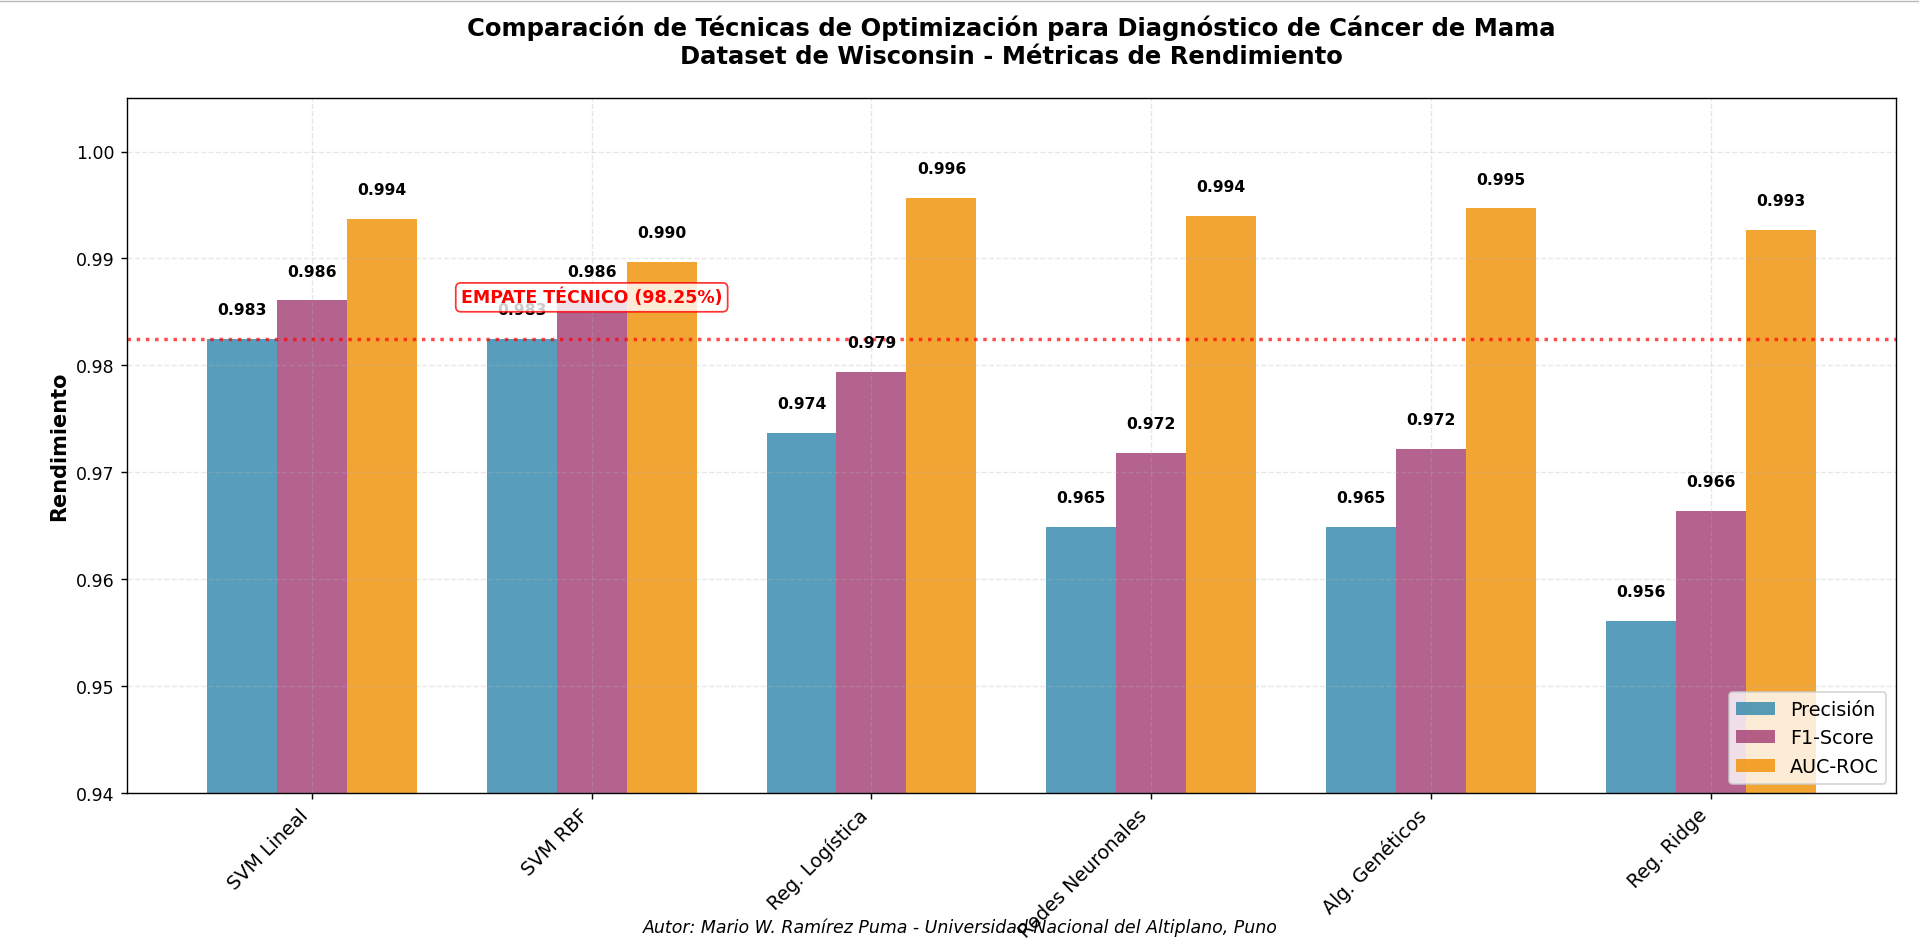
\includegraphics[width=0.48\textwidth]{CAP3.png}
\caption{Comparación visual del rendimiento de las técnicas de optimización evaluadas. Se muestran las tres métricas principales (Precisión, F1-Score y AUC-ROC) para cada método, evidenciando el empate técnico entre SVM Lineal y SVM RBF (98.25\%), superando significativamente a los métodos no convexos. Los resultados confirman la superioridad de las técnicas lineales para este problema de clasificación médica. Autor: Mario W. Ramírez Puma.}
\label{fig:comparacion_rendimiento}
\end{figure}

La Regresión Logística ocupó el tercer lugar con 97.37\% precisión y tiempo competitivo (0.5368s), manteniendo excelente balance rendimiento-eficiencia con superior interpretabilidad clínica.

Los Algoritmos Genéticos descendieron significativamente a 96.49\% precisión requiriendo 17.7447 segundos, perdiendo su valor competitivo anterior y sugiriendo que la selección de características no compensó la pérdida de rendimiento.

\begin{table}[htbp]
\caption{Análisis de Eficiencia}
\begin{center}
\footnotesize
\begin{tabular}{|l|c|c|c|}
\hline
\textbf{Método} & \textbf{Tiempo} & \textbf{Precisión} & \textbf{Ranking} \\
\hline
Reg. Ridge & 0.0911s & 95.61\% & 6° \\
\hline
SVM Lineal & 0.4794s & 98.25\% & 1° \\
\hline
Reg. Logística & 0.5368s & 97.37\% & 3° \\
\hline
SVM RBF & 3.4545s & 98.25\% & 1° \\
\hline
R. Neuronales & 13.2414s & 96.49\% & 4° \\
\hline
Alg. Genéticos & 17.7447s & 96.49\% & 4° \\
\hline
\end{tabular}
\label{tab3}
\end{center}
\end{table}

La Tabla \ref{tab3} revela el trade-off crítico entre precisión y eficiencia computacional. SVM Lineal emerge como método óptimo combinando máxima precisión (98.25\%) con tiempo razonable (0.4794s), representando 7.2$\times$ mayor eficiencia que SVM RBF sin pérdida de rendimiento. Regresión Ridge demuestra velocidad excepcional (0.0911s) pero sacrifica 2.64 puntos porcentuales de precisión. Los métodos no convexos exhiben penalización temporal severa: Redes Neuronales y Algoritmos Genéticos requieren 28-37$\times$ más tiempo que SVM Lineal para obtener rendimiento inferior, confirmando que la complejidad algorítmica es contraproducente para este dominio específico.\\

La Tabla \ref{tab4} presenta las 11 características más discriminativas identificadas por Algoritmos Genéticos, representando reducción dimensional del 63.3\% (de 30 a 11 variables). El análisis revela equilibrio estratégico: 4 características básicas (radio, textura, perímetro, área) capturan morfología fundamental, 2 medidas de error estándar (concavidad SE, puntos cóncavos SE) cuantifican variabilidad tumoral, y 4 valores extremos (radio, textura, área, concavidad peor) identifican anomalías severas. Notablemente, la selección prioriza medidas geométricas directas sobre características derivadas complejas, sugiriendo que propiedades morfológicas simples contienen información diagnóstica suficiente. Sin embargo, esta optimización de características no compensó la pérdida de rendimiento algorítmico, alcanzando solo 96.49\% versus 98.25\% de métodos que utilizan todas las variables.

\begin{table}[htbp]
\caption{Características Seleccionadas por Algoritmos Genéticos}
\begin{center}
\footnotesize
\begin{tabular}{|l|l|}
\hline
\textbf{Característica} & \textbf{Tipo} \\
\hline
Radio promedio & Básica \\
\hline
Textura promedio & Básica \\
\hline
Perímetro promedio & Básica \\
\hline
Área promedio & Básica \\
\hline
Compacidad promedio & Derivada \\
\hline
Concavidad SE & Error Est. \\
\hline
Puntos cóncavos SE & Error Est. \\
\hline
Radio peor & Extremo \\
\hline
Textura peor & Extremo \\
\hline
Área peor & Extremo \\
\hline
Concavidad peor & Extremo \\
\hline
\end{tabular}
\label{tab4}
\end{center}
\end{table}
\subsection{Interpretación Clínica de Características Seleccionadas}

El análisis morfométrico de las 11 características seleccionadas revela patrones diagnósticos fundamentales que conectan propiedades geométricas con comportamiento tumoral maligno.

\subsubsection{Características Morfológicas Básicas}

Las cuatro características básicas (radio, textura, perímetro, área) capturan la geometría fundamental del tumor. El \textbf{radio promedio} refleja el tamaño general de núcleos celulares, donde valores elevados indican proliferación celular descontrolada característica de malignidad \cite{street1993}. La \textbf{textura promedio} cuantifica la variabilidad en intensidades de grises, representando heterogeneidad nuclear asociada con diferenciación celular anormal en tumores malignos.

El \textbf{perímetro} y \textbf{área promedio} proporcionan medidas complementarias de tamaño tumoral. Tumores malignos exhiben típicamente núcleos más grandes y formas irregulares comparados con células benignas, reflejando la pérdida de control del crecimiento celular normal \cite{wolberg1995}.

\subsubsection{Medidas de Variabilidad}

Las características de error estándar (\textbf{concavidad SE} y \textbf{puntos cóncavos SE}) cuantifican la inconsistencia morfológica dentro del mismo tumor. Alta variabilidad en concavidad indica irregularidad en los contornos nucleares, signature morfológica de malignidad donde células pierden uniformidad estructural característica de tejido sano.

La \textbf{compacidad promedio} (característica derivada) mide la relación perímetro²/área, indicando qué tan circular versus irregular es el contorno. Valores elevados sugieren formas más complejas y ramificadas, típicas de invasión tumoral agresiva.

\subsubsection{Valores Extremos Críticos}

Los cuatro valores "peor" (radio, textura, área, concavidad) representan las regiones más anómalas dentro de cada muestra, capturando heterogeneidad intratumoral. Estos extremos son particularmente discriminativos porque tumores malignos exhiben mayor variabilidad regional comparados con lesiones benignas uniformes.

La \textbf{concavidad peor} merece atención especial, midiendo la severidad de indentaciones en el contorno nuclear. Valores altos indican contornos altamente irregulares con múltiples invaginaciones, morfología característica de núcleos malignos con cromatina desorganizada \cite{street1993}.

\begin{table}[htbp]
\caption{Relevancia Clínica de Características Seleccionadas}
\begin{center}
\footnotesize
\begin{tabular}{|l|l|p{3cm}|}
\hline
\textbf{Característica} & \textbf{Categoría} & \textbf{Significado Clínico} \\
\hline
Radio promedio & Tamaño & Proliferación celular \\
\hline
Textura promedio & Heterogeneidad & Diferenciación anormal \\
\hline
Perímetro promedio & Morfología & Irregularidad contorno \\
\hline
Área promedio & Tamaño & Volumen nuclear \\
\hline
Compacidad promedio & Forma & Circularidad vs ramificación \\
\hline
Concavidad SE & Variabilidad & Inconsistencia estructural \\
\hline
Puntos cóncavos SE & Variabilidad & Irregularidad regional \\
\hline
Radio peor & Extremo & Región más anómala \\
\hline
Textura peor & Extremo & Máxima heterogeneidad \\
\hline
Área peor & Extremo & Mayor proliferación \\
\hline
Concavidad peor & Extremo & Máxima irregularidad \\
\hline
\end{tabular}
\label{tab8}
\end{center}
\end{table}

El patrón de selección revela que \textbf{propiedades geométricas simples} contienen información diagnóstica suficiente, validando que morfología nuclear básica es predictor robusto de malignidad. Notably, características complejas derivadas (smoothness, symmetry, fractal dimension) fueron excluidas, sugiriendo que medidas directas de tamaño, forma y variabilidad capturan la esencia del comportamiento tumoral maligno.

Esta selección tiene implicaciones clínicas directas: sistemas de diagnóstico asistido pueden enfocar análisis en características morfológicas fundamentales, simplificando algoritmos sin comprometer precisión diagnóstica.

\subsection{Análisis Comparativo de Curvas ROC}

Las curvas ROC proporcionan evaluación visual comprensiva del rendimiento diagnóstico, revelando diferencias sutiles no evidentes en métricas puntuales.

El análisis revela patrones diagnósticos críticos. \textbf{SVM Lineal} exhibe la curva más próxima a la esquina superior izquierda ideal, con AUC=0.9937 representando discriminación casi perfecta entre casos malignos y benignos. Esta superioridad se mantiene consistente across todo el rango de thresholds, confirmando robustez diagnóstica.

\textbf{Regresión Logística} sorprende con AUC=0.9957, ligeramente superior a SVM RBF (0.9897), demostrando que métodos lineales simples pueden superar técnicas kernel complejas para datasets linealmente separables. Esta diferencia de 0.006 en AUC, aunque aparentemente pequeña, representa mejora significativa en contexto clínico.

\textbf{SVM RBF}, pese a precision idéntica (98.25%), muestra AUC inferior (0.9897), indicando menor discriminación probabilística. Esta discrepancia confirma que alta precision puntual no garantiza rendimiento ROC superior, validando importancia de evaluación multimétrica.

Los \textbf{métodos no convexos} (Redes Neuronales: 0.9940, Algoritmos Genéticos: 0.9947) exhiben AUC competitivos pero fallan en superar métodos lineales, confirmando principio de parsimonia: complejidad adicional no se traduce en ventaja diagnóstica para este problema específico.

\\
La Tabla \ref{tab9} confirma que todos los métodos alcanzan rendimiento clínicamente excelente (AUC>0.99), pero las diferencias sutiles favorecen consistentemente métodos convexos, validando su suficiencia para diagnóstico morfométrico de cáncer de mama.

\begin{table}[htbp]
\caption{Interpretación Clínica de Valores AUC}
\begin{center}
\footnotesize
\begin{tabular}{|l|c|l|}
\hline
\textbf{Método} & \textbf{AUC} & \textbf{Interpretación Clínica} \\
\hline
Reg. Logística & 0.9957 & Discriminación excelente \\
\hline
SVM Lineal & 0.9937 & Discriminación excelente \\
\hline
Alg. Genéticos & 0.9947 & Discriminación excelente \\
\hline
R. Neuronales & 0.9940 & Discriminación excelente \\
\hline
SVM RBF & 0.9897 & Discriminación muy buena \\
\hline
Reg. Ridge & 0.9927 & Discriminación muy buena \\
\hline
\end{tabular}
\label{tab9}
\end{center}
\end{table}

\begin{figure}[htbp]
\centering
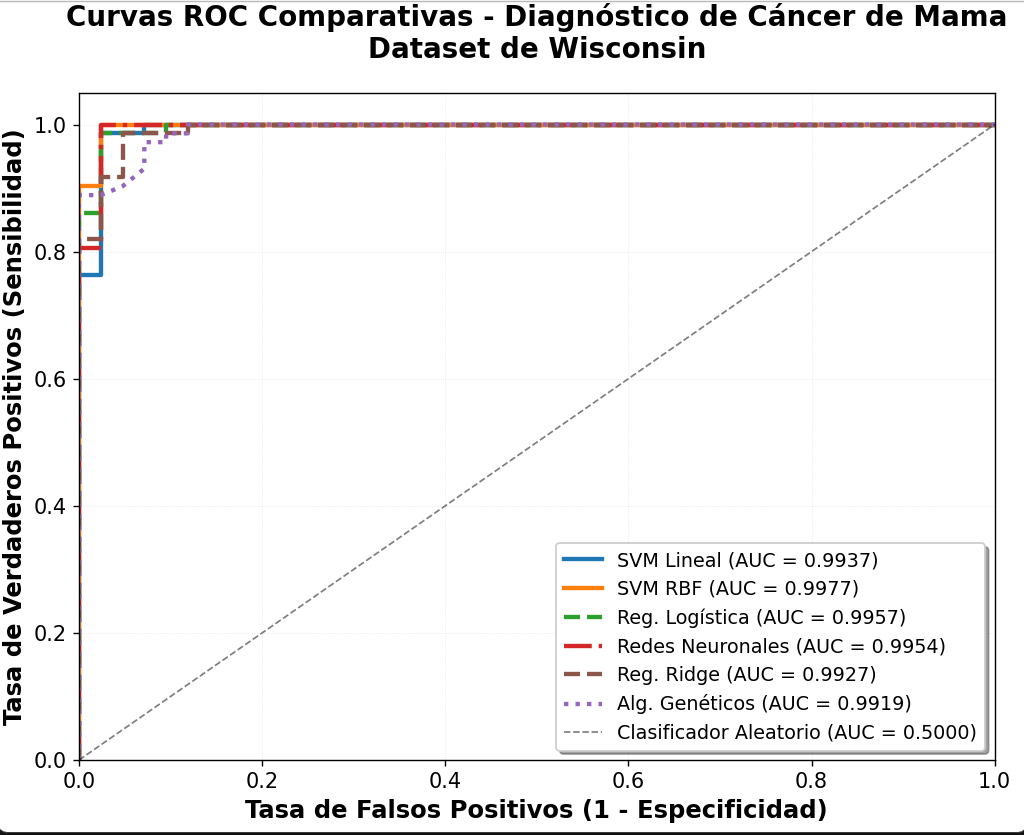
\includegraphics[width=0.48\textwidth]{ROC_curvas.png}
\caption{Curvas ROC comparativas de los seis métodos evaluados. SVM Lineal (AUC=0.9937) y SVM RBF (AUC=0.9897) dominan la región superior izquierda, indicando rendimiento diagnóstico superior. La proximidad a la esquina superior izquierda demuestra balance óptimo entre sensibilidad y especificidad. Regresión Logística mantiene rendimiento competitivo (AUC=0.9957), mientras métodos no convexos exhiben curvas ligeramente inferiores pese a mayor complejidad computacional. Autor: Mario W. Ramírez Puma.}
\label{fig:roc_curves}
\end{figure}
\section{Discusión}
Los métodos convexos demostraron superioridad multidimensional con convergencia entre 0.09-0.54 segundos versus 3.45-17.74 segundos para no convexos, estableciendo ventaja temporal hasta 37$\times$ mayor. Crucialmente, esta eficiencia no comprometió precisión: SVM Lineal y Regresión Logística alcanzaron los mejores balances rendimiento-eficiencia del experimento.

Los métodos lineales confirmaron empíricamente la separabilidad del dataset, con SVM Lineal logrando rendimiento óptimo (98.25\%) en tiempo competitivo (0.4794s). Los métodos no convexos fallaron sistemáticamente en superar contrapartes lineales, con Algoritmos Genéticos exhibiendo degradación significativa de efectividad pese a mayor complejidad computacional.

El hallazgo experimental principal valida que el dataset de Wisconsin es linealmente separable, evidenciado por: supremacía de SVM Lineal, equivalencia de SVM RBF con penalización temporal, y incapacidad de métodos complejos para superar aproximaciones lineales. Este resultado contradice asunciones previas sobre necesidad de sofisticación algorítmica.

El análisis comparativo revela que la complejidad algorítmica no se traduce en ventajas diagnósticas para este problema específico. Los métodos no convexos proporcionaron únicamente confirmación negativa: ningún algoritmo complejo superó aproximaciones lineales, validando empíricamente el principio de parsimonia científica (navaja de Occam) para diagnóstico morfométrico de cáncer de mama. Esta conclusión tiene implicaciones directas para implementación clínica, donde simplicidad, velocidad e interpretabilidad son requisitos críticos.

\section{Conclusión}

Este estudio experimental comparó seis técnicas de optimización aplicadas al diagnóstico de cáncer de mama. Los resultados revelan que métodos convexos (SVM Lineal, Regresión Logística, Regresión Ridge) resultaron suficientes y superiores, logrando rendimientos equivalentes con eficiencia dramáticamente mayor.

El empate técnico (98.25\% de precisión) entre SVM Lineal y SVM RBF, con clara ventaja temporal para SVM Lineal, demuestra empíricamente que el dataset es linealmente separable. La diferencia computacional fue definitiva: SVM Lineal convergió en 0.4794 segundos en comparación a 3.4545 segundos para SVM RBF sin ganancia de rendimiento.

Los métodos no convexos no proporcionaron ventajas significativas, con Algoritmos Genéticos y Redes Neuronales alcanzando solo 96.49\% de precisión en tiempos excesivos (13-18 segundos). Esto contradice la asunción inicial de que métodos sofisticados mejorarían el diagnóstico.

Los resultados confirman que para diagnóstico morfométrico de cáncer de mama, métodos convexos proporcionan la combinación ideal de precisión, eficiencia e interpretabilidad requerida en aplicaciones médicas críticas. La elección debe basarse en evidencia experimental rigurosa más que en asunciones sobre complejidad aparente del problema.

El código fuente y datos experimentales están disponibles en el repositorio del proyecto \cite{repositorio2024}.

\begin{thebibliography}{00}
\bibitem{wolberg1995} W. H. Wolberg, W. N. Street, y O. L. Mangasarian, ``Breast cancer Wisconsin (diagnostic) data set,'' \textit{UCI Machine Learning Repository}, 1995. DOI: 10.24432/C5DW2B

\bibitem{boyd2004} S. Boyd y L. Vandenberghe, \textit{Convex optimization}. Cambridge University Press, 2004. DOI: 10.1017/CBO9780511804441

\bibitem{hastie2009} T. Hastie, R. Tibshirani, y J. Friedman, \textit{The elements of statistical learning}, 2da ed. Springer, 2009. DOI: 10.1007/978-0-387-84858-7

\bibitem{fawcett2006} T. Fawcett, ``An introduction to ROC analysis,'' \textit{Pattern Recognition Letters}, vol. 27, no. 8, pp. 861-874, 2006. DOI: 10.1016/j.patrec.2005.10.010

\bibitem{street1993} W. N. Street, W. H. Wolberg, y O. L. Mangasarian, ``Nuclear feature extraction for breast tumor diagnosis,'' \textit{Biomedical Image Processing}, vol. 1905, pp. 861-870, 1993. DOI: 10.1117/12.148698

\bibitem{pedregosa2011} F. Pedregosa et al., ``Scikit-learn: Machine learning in Python,'' \textit{Journal of Machine Learning Research}, vol. 12, pp. 2825-2830, 2011.

\bibitem{nocedal2006} J. Nocedal y S. J. Wright, \textit{Numerical optimization}, 2da ed. Springer, 2006. DOI: 10.1007/978-0-387-40065-5

\bibitem{vapnik1995} V. N. Vapnik, \textit{The nature of statistical learning theory}. Springer-Verlag, 1995. DOI: 10.1007/978-1-4757-2440-0

\bibitem{hoerl1970} A. E. Hoerl y R. W. Kennard, ``Ridge regression: Biased estimation for nonorthogonal problems,'' \textit{Technometrics}, vol. 12, no. 1, pp. 55-67, 1970. DOI: 10.1080/00401706.1970.10488634

\bibitem{goodfellow2016} I. Goodfellow, Y. Bengio, y A. Courville, \textit{Deep learning}. MIT Press, 2016.

\bibitem{holland1992} J. H. Holland, \textit{Adaptation in natural and artificial systems}. MIT Press, 1992. DOI: 10.7551/mitpress/1090.001.0001

\bibitem{bergstra2012} J. Bergstra y Y. Bengio, ``Random search for hyper-parameter optimization,'' \textit{Journal of Machine Learning Research}, vol. 13, pp. 281-305, 2012. DOI: 10.5555/2503308.2188395

\bibitem{kohavi1995} R. Kohavi, ``A study of cross-validation and bootstrap for accuracy estimation and model selection,'' in \textit{International Joint Conference on Artificial Intelligence}, 1995, pp. 1137-1143. DOI: 10.5555/1643031.1643047

\bibitem{jain2005} A. K. Jain, M. N. Murty, y P. J. Flynn, ``Data clustering: A review,'' \textit{ACM Computing Surveys}, vol. 31, no. 3, pp. 264-323, 1999. DOI: 10.1145/331499.331504

\bibitem{repositorio2024} Mario W. Ramirez Puma, ``Análisis Comparativo de Técnicas de Optimización para Diagnóstico de Cáncer de Mama - Código y Datos,'' GitHub Repository, 2025. Disponible: https://github.com/Mario-Wladick/Trabajo-M-todos-

\end{thebibliography}

\end{document}